\documentclass[../main.tex]{subfiles}
\graphicspath{{\subfix{../images/}}}

\begin{document}
	\chapter{Scelte organizzative}

	\section{Introduzione}
	Ora analizzeremo alcune scelte che stanno alla base del organizzazione dei sistemi informativi nelle aziende.
	\begin{itemize}
		\item Le forme di reperimento/costruzione del sistema informativo.
		\item I tipi di figure informatiche.
		\item Le scelte strategiche sull'infrastruttura.
		\item Le problematiche legate all'unteroperabilità del servizio fornito dal sistema.
	\end{itemize}

	\section{Costruzione del sistema informativo}
	Al giorno d'oggi esistono tre modalità:
	\begin{enumerate}
		\item \textbf{Make: } costruire interamente il proprio sistema informativo.
		\item \textbf{Buy: } comprarlo dall'esterno.
		\item \textbf{Outsource: } darlo in gestione ad un'ente esterna.
	\end{enumerate}
	Nel mondo reale però non si adotta una sola tecnica ma solitamente si punta a mescolarle.

	\subsection{Make}
	Questa scelta molto in voga alla nascita dei primi sistemi informativi è oggi usata solo da grandi aziende.\\
	Con questa opzione l'azienda sviluppa tutto il software necessario e i servizi, l'unica cosa comprata dall'esterno per ovvi motivi è l'hardware.
	\begin{itemize}
		\item Costi fissi molto alti: l'azienda deve possedere uno staff preposto allo sviluppo e alla gestione di tale software.
		\item Investimenti consistenti: oltre all'acquisto di tutta l'infrastruttura per poter lavorare l'azienda deve anche comprare hardware ed eventuale software.
		\item Struttura che non si confronta col mercato: uno degli aspetti più critici, essendo il software in una specie di "monopolio" per l'azienda che lo ha prodotto non è soggetto a nessun miglioramento dato dalla competizione del mercato.
		\item Le soluzioni tendono a diventare obsolete: questa problematica è fortemente legata alla precedente.
		\item Tempi di soluzione veloci per problemi banali ma molto dilatati per problemi complessi.
		\item Mantenimento interno del "know-how": ovvero solo l'azienda sa come funziona il software che ha prodotto quindi in casi di riservatezza molto alta questo risulta essere un punto a favore non da poco.
		\item I modelli organizzativi sono mappati in modo molto puntuale perchè il software è sviluppato ad-hoc, questo però non è sempre un vantaggio in quanto molte volte le soluzioni più generali risultano essere molto più efficenti.
	\end{itemize}

	\subsection{Buy}
	Questa scelta prevede l'acquisto del proprio SI da un'azienda specializzata ed esterna, solitamente questa scelta era adottata da molte PMI ma con l'introduzione degli ERP anche dalle grandi aziende.
	\begin{itemize}
		\item E' comunque presente, seppur in dimensioni ridotte, una struttura interna all'azienda per poter dialogare e sincronizzare i fornitori.
		\item Parziale smobilizzazione degli investimenti iniziali dell'azienda infatti non viene pagato lo sviluppo del software.
		\item Concetrazione sul core business: non dovendo pensare allo sviluppo del SI.
		\item Dipendenza da una struttura esterna, solitamente i tempi necessari per cambiare fornitore sono molto lunghi e le software house detengono molto potere contrattule.
		\item Maggior flessibilità rispetto al "make", un fonrnitore essendo sul mercato deve avere una dimensione adeguata per poter seguire i propri clienti.
		\item Fuoriuscita di parte del "know-how" aziendale: per necessità la software house dev conoscere i processi e i dati interni di un'azienda.
		\item Mancanza di proprietà del software: tutte le spese connesse ad un software non portano alla proprietà di esso, solamente alla detenzione di una licenza di uso.
		\item Possibilità di interventi limitata: ovviamente se insorgono problemi deve essere il fornitore ad occuparsene e non l'azienda direttamente.
		\item Continua aderenza al mercato essendo il fonitore immerso nel mercato.
		\item Modelli organizzativi mediati: solitamente la software house ha la propria soluzione che deve essere personalizzata per l'azienda.
		\item Difficoltà nell'interazione con più fornitori: spesso dialogare con molti fornitori per poter opeare sul sistema informativo da loro comprato è dispendioso di risorse.
	\end{itemize}
	\begin{center}
		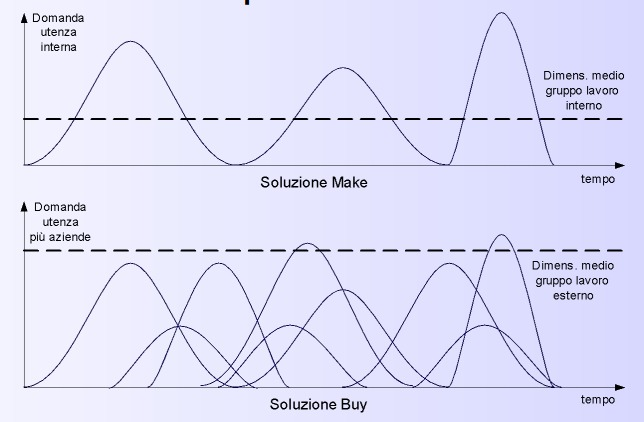
\includegraphics[scale=0.5]{opzione_buy.png}
	\end{center}
	
	\subsection{Outsource}
	Questa scelta organizzativa consiste nel portare all'esterno tutto quello ch riguarda lo sviluppo/gestione/mantenimento del sistema informativo, pagando un canone mensile opper con tempi più lunghi.\\
	Si noti che l'outsourcing è concettualmente diverso dal hosting in cui si porta all'esterno l'infrastryttura ma si mantiene il controllo del softwre che solitamnete è gestito con la "buy" e dal body-rental in cui si affitta il personale di un'altra azienda nei periodi i maggior richiesta.
	L'opzione "outsource" inizialmente circoscritta alle grandi aziende è ad oggi usata da molte PMI, possiamo trovare sistemi in outsourcing completo nelle grandi aziende oppure soluzioni parziali nelle PMI.\\
	La crescentre complessità dei sistemi ed il bisogno di garantire sicurezza e continuità rendono pocco conveniente creare un servizio all'interno di un'azienda.
	\begin{itemize}
		\item Costi variabili: non essendoci personale dedicatio i costi risultano fissi, a meno di cambio del canone di utilizzo.
		\item Smobilizzazione totale degli investimenti: non essendoci alcun investimento in infrastruttura, hardware e software.
		\item Voncolo completo con il fornitore del servizio, se il fornitore chiudesse l'azienda sarebbe privata del proprio SI.
		\item Maggior flessibilità rispetto al "make" perchè è spesso presente una possibilità di scalare i servizi ricevuti.
		\item Esposizione di tutto il know-how perchè completamente affidato a terzi.
		\item Perdita di controllo sulla potenza contrattuale che un fornitore può esercitare sull'azienda.
		\item Possibilità di intervento diretto assente.
		\item Esattamente come nel modello "buy" si è molto più aderenti al mercato e con modelli organizzativi mediati.
	\end{itemize}

	\section{Posizionamento del sistema informativo}
	\subsection{Figure professionali}
	Le figure professionali "informatiche" che operano all'interno di un'azienda sono legate alla "maturità informatica" che un azienda possied,
	possiamo considerarne quattrio livelli.

	\subsubsection{Livello 1}
	Il team è composto da un ristretto numero 
\end{document}